

\subsection{Balancing, Texte und Story: Spieldesign}



\subsubsection{Spieldesign} Am Anfang der Entwicklung musste ein geeignetes Setting für das geplante RPG gefunden werden. Zur Auswahl standen die beiden klassischen, den meisten bekannten Arten von Spieleuniversen zur Auswahl. Das eine wäre futuristisches Scifi und das andere eher mittelalterliches Fantasy. 

In der Frühen Phase der Entwicklung war beim Spieldesign ursprünglich geplant ein RPG zu entwickeln, dass viele Elemente des klassischen Pen and Paper Rollenspielen, wie z.B. Dungeons \& Dragons enthält. Man wollte unterschiedliche Charakterklassen, die sich in ihrer Ausrüstung, wie individuelle Waffen und Rüstungen, sowie ihren spezifischen Fähigkeiten klar voneinander unterscheiden. Ein Levelsystem, bei dem die einzelnen Charaktere von Abenteuer zu Abenteuer ihre Fähigkeiten verbessern und bessere Ausrüstung in Form von Beutegut finden können, sollte auch enthalten sein. Das Entwicklerteam hat sich dann für das Fantasy Setting entschieden, weil man der Ansicht war, dass sich die vorher genannten Eigenschaften damit besser umsetzen lassen würden. Speziell die unterschiedlichen Eigenschaften der Charakterklassen waren bei dieser Entscheidung maßgeblich, denn eine Eingrenzung auf die besonderen Fähigkeiten der unterschiedlichen Spielfiguren, wie z. B. einen Tank\footnote{Eine in Spielen übliche Bezeichnung für eine Charakterklasse, die sich durch eine besonders Starke Rüstung, Ausdauer und/oder Verteidigung auszeichnet.}, einen Healer\footnote{s. vorgen., hier aber eine Charakterklasse die die Lebenspunkte durch Heil-Zauber wiederherstellen kann.} und einen Damagedealer\footnote{s. vorgen., ist eine Charakterklasse die besonders viel Schaden verursachen kann.}, schien im Scifi-Hintergrund nicht so einfach und für den Spieler nicht schlüssig zu gestalten.

\begin{figure}[H]
    \centering
    \caption{Details den Klassen aus der Projektbesprechung vom 11.12.2021}
    \label{fig:2021-12-11-Projekt-Besprechung-Klassenbeschreibung}
    \fbox{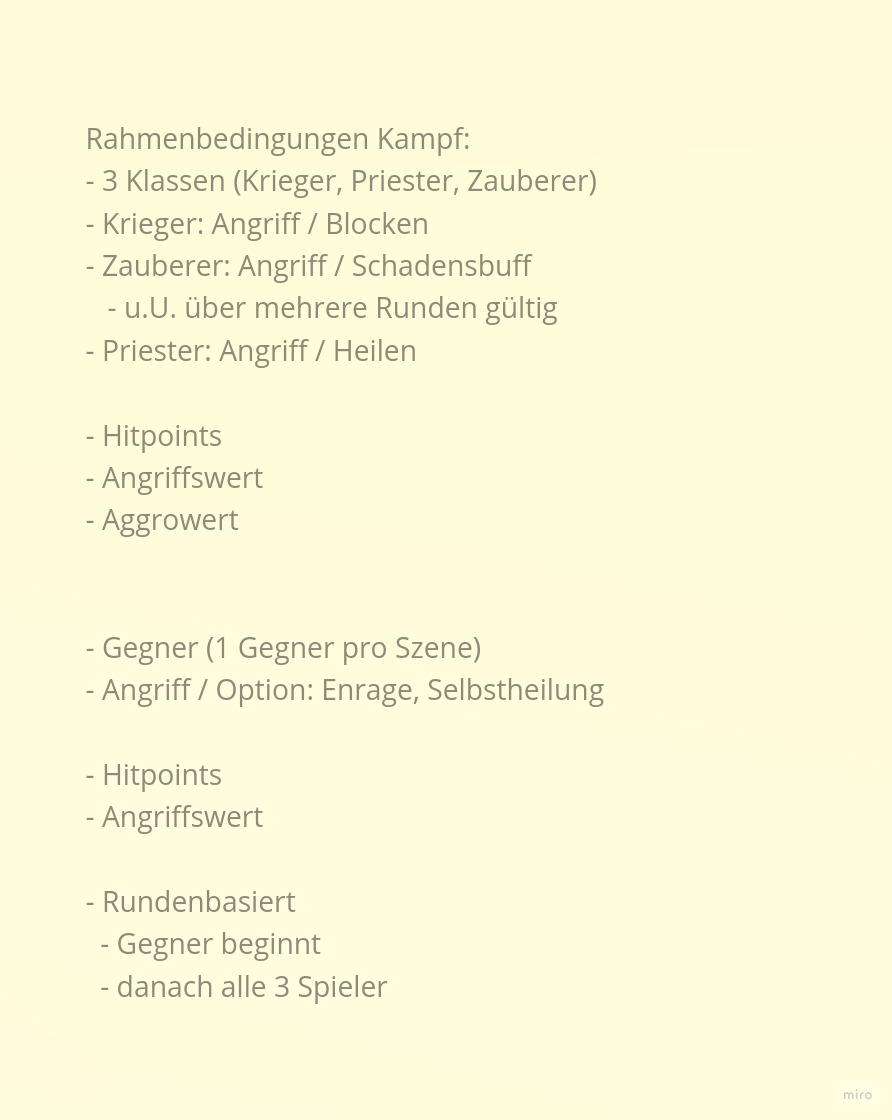
\includegraphics[width=0.5\textwidth]{2021-12-11-Projekt-Besprechung-Klassenbeschreibung}}
\end{figure}


Die Überlegungen führten somit schon am Anfang recht schnell zu den bereits erwähnten unterschiedlichen Spielfiguren, die der Spieler verkörpern kann. Ein Tank soll Schaden von anderen und sich selbst abhalten können. Ein Heiler soll sich und seine Kameraden heilen können und ein Damagedealer soll seinen Schaden und den der anderen Spielfiguren erhöhen. Es war angedacht, dass die einzelnen Spielfiguren über Lebenspunkte, Magiepunkte und verschiedene Handlungsoptionen verfügen, die sich abhängig von der Charakterklasse, voneinander unterscheiden. Auch schien klar zu sin, dass die Würfelmechanik, die Pen and Paper Rollenspielen zu Grunde liegt in das Spiel übernommen werden soll.

Das Spiel sollte vom Ablauf her, aus aufeinander aufbauenden Abenteuern bestehen, die die Charaktere gemeinsam erleben und die mit Hilfe von unterschiedlichen Ansätzen gelöst werden können, bestehen. Dazu sollten sie sich gemeinsam durch eine grafisch animierte Spielwelt bewegen.

Es war geplant als Grundlage für die Regeln, denen das Spiel folgen, also wie ist zu bestimmen, wie und in welcher Reihenfolge der Kampf abläuft oder zu welchen Bedingungen genau wird bestimmt, wann z. B. ein Schwerthieb trifft oder nicht, dass sollte auf Grundlage der Opensource License von dem Rollenspiel Dungeons and Dragons 3.5 basieren.

Nachdem dieser grobe Ramen festgelegt wurde, haben wir entschieden erst einmal einen Prototypen zu entwickeln, der exemplarisch anhand eines Abenteuers, im Folgenden nur noch Spielszene oder Szene genannt, zu klären ob der gesetzte Ramen auch so umsetzbar ist. 

Dabei ist recht schnell aufgefallen, dass vor allem die geplanten unterschiede der einzelnen Charakterklassen, in Form von sich unterscheidenden Handlungsmöglichkeiten in der Szene nicht klar abzugrenzen ist. Außerdem war nicht klar, wie es zu handhaben ist, wenn man z. B. vor einer verschlossenen Tür steht, diese zu öffnen ist, und jede Charakterklasse eine andere Möglichkeit hat dieses Hindernis zu überwinden. 

Wenn auch bei diesem einfachen Beispiel recht einfach zu klären ist, wie die unterschiedlichen Handlungsmöglichkeiten aussehen, nämlich "Tür eintreten", "Schloss knacken" und die Tür mit einem Zauber öffnen, war nicht klar wie genau das ablaufen sollte. Wer z. B. darf den in diesem Moment die Handlung bestimmen? Derjenige, der zuerst auf den Button klickt? Und was geschieht danach, entsprechend der unterschiedlichen Auswahl der Möglichkeiten? Sollte alles zu unterschiedlichen Ergebnissen führen oder alles zur selben? Dieses würde wiederum die Auswahl, was zu tun ist, völlig unnötig machen. Und falls die Auswahl zu unterschiedlichen Ergebnissen führt, entsteht ein für uns nicht einzuschätzender Aufwand an Storytelling, grafischen Animationen und an Programmierbarkeit. Außerdem ist die Komplexität der Kampfmechanik, wie sie in dem zu Grunde liegenden Regelsystem von Dungeons \& Dragons 3.5 recht anspruchsvoll und für einen gemütlichen Abend mit seinen Freunden und auf das Spielen von Angesicht zu Angesicht im Real Live ausgelegt. Dies ermöglicht eine andere Spielweise als allein vor einem PC. Zum Beispiel kann sich ein Charakter aus dem Kampf zurückziehen oder ein anderer aus der Abenteurergruppe nimmt seinen Platz in der Kampflinie ein. Der Spielleiter, der die Gegner steuert, kann auch entscheiden einen anderen Charakter anzugreifen, wenn er den Eindruck hat, dass sonst der Charakter stirbt. Dies sind alles Mechaniken, die zwar zu programmieren sind, aber würde sie den Ramen für das erste Projekt in dieser Art sicher sprengen.
Außerdem besteht ein Charakter in diesem Regelwerk aus vielen Eigenschaften, die in Zahlenwerten festgehalten werden. All diese Werde beeinflussen wie er z.B. kämpfen, stehlen oder mit anderen Menschen interagieren kann. Jeder Gegenstand, der als Beutegut von den Charakteren gefunden wird, hat Auswirkungen darauf. Dies ist nur eine grobe Zusammenfassung der Dinge, die die Regelmechanik beeinflussen und auch große Spieletitel wie z.B. Baldursgate, die ebenfalls auf Dungeons \& Dragons 3.5 basieren, haben nicht das gesamte Regelwerk übernommen. 

Auf Grund all der oben genannten Unwägbarkeiten und Komplexität haben wir uns an diesem Punkt zu einer, im Folgenden erklärten, Konzeptänderung entschieden.

Der gravierendste Schritt ist sicher, dass aus dem RPG eine Art Beat em Up mit Fantasy Hintergrund und atmosphärischen Texten und Grafiken geworden ist. Dabei gibt es zwar noch immer einzelne Level, die man durchspielt, diese sind aber recht linear und bestehen nur aus einem Kampf gegen einen Gegner, den man entweder gewinnt oder verliert. Es wird Szenen geben, die nur allein zu Spielen sind und Szenen, die mehrere Spieler benötigen. Ganz grob soll es so ablaufen.

Am Anfang der Szene wird ein Hintergrundbild mit Texterklärung eingeblendet und nachdem die oder der Spieler bestätigt haben, wechselt die Ansicht. Nun sieht man eine Abbildung der Szene mit dem Gegner. Rechts davon befindet sich das Kampflog und den Chat, darunter den Status der Spieler. Je nach Ausgang des Kampfes wird ein anderer Outrotext angezeigt und man springt nach dem Kampf zurück in die Auswahl für neue Kämpfe. Es wird keine Ausrüstung geben, die die Charaktere finden können, denn jeder gefundene Gegenstand sollte unterschiedliche Eigenschaften haben und sich in irgendeiner Weise Auf den Charakter auswirken. Dies hätte zu diesem Zeitpunkt der Entwicklung zu einem zu umfangreiches Datenbankmanagement, für das von uns anvisierte Ziel, geführt. Das Konzept, dass ein Charakter seine Eigenschaften verbessert, in dem er bei den Kämpfen an Erfahrung gewinnt, besteht weiterhin, wenn auch etwas einfacher als angedacht. Auch ist es so geblieben, dass sich jede Charakterklasse von der anderen durch eine Spezialfähigkeit unterscheidet. Die Klassen sind ebenfalls geblieben nur hat sich die Bezeichnung etwas konkretisiert. Im Einzelnen sind das der Kämpfer, er hat die Möglichkeit den erhaltenen Schaden zu reduzieren. Dann gibt es noch den Priester, der die Fähigkeit hat zu Heilen und dann ist da noch der Magier, der den Schaden erhöhen kann. Nach jedem Kampf gibt eine individuelle Summe an Erfahrung, die dem Charakter gutgeschrieben wird, die er dazu benutzen kann die Fähigkeiten seines Charakters zu verbessern. Der Spieler kann mit der erhaltenen Erfahrung die Lebenspunkte (HP) oder die Angriffskraft (AP) seines Character steigern. Ein Charakter erhält immer Erfahrung, egal ob der Kampf gewonnen wird oder verloren geht. Bei einem Sieg ist diese jedoch deutlich höher als bei einer Niederlage. Das hat zur Folge das man einen Level eventuell mehrfach spielen muss, um den nächsten Level erfolgreich abschließen zu können. Der Mechanismus des Würfelns ist ebenfalls in der Art implementiert, dass nicht jeder Treffer einen festen Schaden zufügt, sondern es gibt einen Minimum- und einen Maximumschaden, der zufällig zwischen beiden Extremen errechnet wird. Der endgültige Tod eines Charakters ist nicht vorgesehen. 

Die Kampfmechanik wird wie folgt aussehen. Der Kampf ist deutlich vereinfacht und wird Rundenbasiert ablaufen, wobei in jeder Runde der Gegner zuerst angreift. Danach wird jeder Charakter die Möglichkeit haben entweder anzugreifen oder seine Spezialfähigkeit einzusetzen oder auszusetzen. Falls der Charakter seine Spezialfähigkeit nutzt, kann er nicht angreifen und umgekehrt. Die Spezialfähigkeit wirkt mehrere Runden nach. Es ist nicht vorgesehen zu testen, ob ein Angriff trifft oder nicht, ein Angriff trifft also immer und macht Schaden. Der Gegner verfügt über keine Spezialfähigkeiten. Macht dieser Schaden, so wird ein Spieler ausgewählt, dem dann der spezifischen Schaden zugefügt wird. D. h. der Warg der z. B. 20 Punkte Schaden pro Angriff macht, fügt dem ausgewählten Charakteren die 20 Punkte Schaden zu. Der Schaden der Spieler summiert sich, so dass drei Spieler die jeweils 20 Schaden zufügen, dem Warg also in Summe 60 Punkte Lebensenerie abziehen. Vor jedem neuen Kampf verfügen die Spieler wieder über ihre vollen Lebenspunkte (HP).

\subsubsection{Balancing} Trotz der recht einfachen Mechanik ist das Ballancing doch recht komplex, denn die einzelnen Klassen, unterscheiden sich klar in ihren Fähigkeiten von einander und sollen trotzdem ihrer unterschiedlichen Spielweise ungefähr gleichwertig im Spiel sein und dem Spieler natürlich auch gleich viel Spaß bereiten. Um dafür die richtigen Stellschrauben zu haben, damit die Fähigkeiten, Lebenspunkte (HP) und Angriffspunkte (AP) individuell eingestellt werden können, sind sämtliche Werte so hinterlegt, dass sie einzeln abgeändert werden können. Im Einzelnen stellt sich das wie folgt dar. 

Wie schon erwähnt, können HP und AP für jede Klasse und jeden Gegner einzeln und völlig unabhängig voneinander abgeändert werden. Die Spezialfähigkeiten der einzelnen Charakterklassen sind in Dauer und Ausprägung unterteilt, die sich wie bei den anderen Werten individuell für jede Klasse einzeln regeln lassen. Auch die erhaltene Erfahrung ist mit einem abänderbaren Multiplikator versehen, um Einfluss darauf zu nehmen wie viel Erfahrung die einzelnen Charaktere erhalten und damit wie schnell sie ihre Fähigkeiten verbessern können. Dabei ist ebenfalls darauf geachtet worden, dass es die Möglichkeit gibt, dass HP und AP unterschiedlich viele Erfahrungspunkte kosten können und wie alle anderen Werte ist dies auch variabel einstellbar. Die unterschiedlichen Erfahrungspunktkosten von HP und AP sind nötig, weil der Unterschied von diesen die Charaktere voneinander abgrenzt und diese im Kampf unterschiedlich wichtig sind und die Spieler nicht zu schnell zu mächtig werden sollen.

\begin{lstlisting}
"name": "ability_m_effect_strength",
"type": "float", "value": "0.6",
"hint": "strength of the mage ability in percent (written in float, 0.1 = 10%, 0.5 = 50%)"

"name": "ability_m_duration_rounds",
"type": "int", "value": "2",
"hint": "mage ability will be applyed to this number of next rounds"

"name": "ability_p_effect_strength",
"type": "float", "value": "0.08",
"hint": "strength of the priest ability in percent (written in float, 0.1 = 10%, 0.5 = 50%)"

"name": "ability_p_duration_rounds",
"type": "int", "value": "4",
"hint": "priest ability will be applyed to this number of next rounds"

"name": "ability_w_effect_strength",
"type": "float", "value": "0.20",
"hint": "strength of the warrior ability in percent (written in float, 0.1 = 10%, 0.5 = 50%)"

"name": "ability_w_duration_rounds",
"type": "int", "value": "3",
"hint": "warrior ability will be applyed to this number of next rounds"
\end{lstlisting}

Die Trennung von HP und AP hat außerdem zur Folge, dass nicht jeder Charakter, derselben Klasse, demselben Stereotyp entspricht. Also ist es möglich, dass sich jeder Krieger, so der Spieler denn möchte, anders entwickeln kann als der Krieger, den der Spieler davor gespielt hat. Der Spieler kann also einen Krieger erschaffen, der entweder Wert auf HP oder AP legt und das jedes Mal individuell neu entscheiden. Dies Gilt auch für alle anderen Klassen. Der variable Schaden soll dazu dienen, dass nicht jeder Kampf vorherberechnet werden kann, indem man die HP des Gegners mit den AP des Spielers vergleicht.

All das führt dazu, dass das Ballancing gut und kleinschrittig angepasst werden kann, macht es aber aufgrund der vielen Stellschrauben auch sehr komplex und für uns, die wir über wenig Erfahrung im Spielebalancing verfügen, auch schwierig alles aufeinander anzustimmen. Die im veröffentlichten Spiel festgelegten Werte stellen einen Kompromiss aus Arbeitsaufwand und Spielbarkeit bzw. Spielerfahrung dar. Diese könnten noch durch ein umfangreiches Betatesting, dass üblicherweise an so einem Punkt bei Spieleentwicklern geschieht, optimiert werden. Dafür gibt es hier aber weder Zeit noch Ressourcen, um die Rückmeldungen von einer Vielzahl von Testern auszuwerten und in die Entwicklung einfließen zu lassen und anschließend nochmals zu Prüfen ob die Änderungen zu den gewünschten Ergebnissen geführt haben. Beim Ballancing des Spiels hat sich außerdem gezeigt, dass die Teilbereiche Programmierung und Ballancing unbedingt eng zusammenarbeiten sollten, damit die nötigen Mechaniken auch vorhanden sind und nicht noch nachträglich evtl. umständlich implementiert werden müssen, wenn das zu diesem Zeitpunkt dann überhaupt noch möglich ist.

\subsubsection{Storytelling} Am Anfang war generell festzulegen in welcher Sprache das Spiel erscheinen soll, dabei standen Englisch und Deutsch zur Auswahl und ursprünglich sollte das Spiel auf Englisch erscheinen und die ersten Konzeptzeichnungen der Charakterbeschreibungen wurden auch in englischer Sprache verfasst. Aufgrund von Vereinfachung, da jeder der Entwickler Muttersprachler in Deutsch ist, wurde auch hier eine Änderung hin zur deutschen Sprache vollzogen. Außerdem wird das Spiel nur im Zusammenhang mit einer Studienarbeit entwickelt und soll im deutschsprachigen Raum veröffentlicht werden. Um die Entwicklung nicht unnötig auf Grund von sprachlichen Schwierigkeiten zu verkomplizieren, schien dieser Schritt logisch. 

Die Entwicklung hin zu einem Spiel, in dem die Level oder Spielszenen nur lose zusammenhängen, machen es nötig zu jeder einzelnen Szene eine Story zu schreiben, um dem Spieler ein Gefühl zu geben, was gerade passiert und warum. Außerdem sind unterschiedliche Texte je nach Ausgang der Spieleszene vorgesehen und unterschiedliche Texte, die z.B. beschreiben was gerade im Kampf geschieht. Dabei ist es wichtig sich auf die Beschreibung der dargestellten Szene zu konzentrieren und nicht abzuschweifen, da ein zu langer Text vom Spieler vielleicht nicht gelesen wird oder als störend empfunden wird. Jedoch muss er lang und intensiv genug sein, damit sich der Spieler einen Eindruck von dem Geschehen verschaffen und darin eintauchen kann. Schließlich soll das Spiel auch eine Geschichte erzählen und dem Spieler eine gewisse Spielerfahrung und im Idealfall einen Wiederspielwert geben. 

Beim Entwickeln der einzelnen Szenen ist aufgefallen, dass man nicht immer genau sagen kann, was zuerst da war, das Huhn oder das Ei, denn der Text und die Grafik stehen in engem Zusammenhang und haben sich gegenseitig beeinflusst. Die Beschreibung der Szene stand üblicherweise zuerst und danach wurde die Szenengrafik entwickelt. Aber manchmal war es auch umgekehrt oder es war nötig den Text anzupassen, weil die Animation z. B. eines Rudels Wölfe schwieriger war als die von einem einzigen riesigen Wolf. So wurde aus dem Rudel Wölfe was die Gegend terrorisiert ein einziger großer Warg. Oder im Fall der Szene im Anwesen war bei ursprünglicher Planung ein Geist vorgesehen, aber beim Schreiben der Geschichte wurde daraus ein Vampir, der viel düsterer ist und sinniger passt.

Daraus ist zu erkennen, dass bei einer Spieleentwicklung diese beiden Teilbereiche sehr eng zusammenarbeiten sollten. Dem Programmierer z. B. ist es egal, oder wie unser Leadprogrammer sagte "Ich bin da total leidenschaftslos", was für eine Grafik oder Text an entsprechender Stelle im Code eingefügt werden. Aber Texte und Grafik müssen unbedingt Hand in Hand gehen und sich gegenseitig ergänzen, um eine überzeugende Spielerfahrung zu schaffen. 

Im Fall des Kampfes gegen den Drachen und den Vampierlord ist man bewusst von der reinen Beschreibung der Szene abgewichen und hat viel mehr die Motivation des Charakters und etwas Hintergrundgeschichte in den Vordergrund gestellt, um beim Spieler die Beweggründe des Charakters in den Vordergrund zu stellen, damit sich dieser, nicht wie bei den anderen Szenen, in Handlung sondern mehr in den Akteur hinein versetzen kann. Bei diesen Gegnern sollte auch etwas Besonderes im Text stehen, außerdem wollte der Autor auch unterschiedliche Arten der Erzählung ausprobieren.
